\documentclass[12pt]{article}
\usepackage{amsmath,amsfonts,amsthm,amssymb}
\usepackage{setspace}
\usepackage{fancyhdr}
\usepackage{lastpage}
\usepackage{extramarks}
\usepackage{enumitem}
\usepackage[ruled,vlined]{algorithm2e}
\usepackage{chngpage}
\usepackage{soul,color}
\usepackage{graphicx,float,wrapfig}
\usepackage{listings}
% \usepackage{algorithmic}
\pagestyle{empty}
\usepackage{tikz}
\usetikzlibrary{decorations.markings}
\usetikzlibrary{quotes}
\tikzstyle{vertex}=[circle, draw, inner sep=0pt, minimum size=6pt]
\newcommand{\vertex}{\node[vertex]}
\addtolength{\textwidth}{20mm}
\addtolength{\oddsidemargin}{-10mm}
\addtolength{\textheight}{30mm}
\addtolength{\topmargin}{-14mm}
\newcommand{\Class}{ \normalsize CS 331: Algorithms and Complexity (Spring 2024)\\
\small    Unique Number: 50930, 50935 50940, 50945
}
%\newcommand{\ClassInstructor}{Fares}
% Homework Specific Information. Change it to your own


\def\changemargin#1#2{\list{}{\rightmargin#2\leftmargin#1}\item[]}
\let\endchangemargin=\endlist

%\newcommand{\ClassInstructor}{Fares}
%\newcommand{\ClassInstructor}{Fares}

\def\changemargin#1#2{\list{}{\rightmargin#2\leftmargin#1}\item[]}
\let\endchangemargin=\endlist


%\newcommand{\ClassInstructor}{Fares}
% Homework Specific Information. Change it to your own
\newcommand{\Title}{Assignment 6 - Solution}
\newcommand{\DueDate}{Tuesday, 19 March, by 11.59pm}

\newcommand{\StudentName}{}
\newcommand{\StudentClass}{}
\newcommand{\StudentNumber}{}

% In case you need to adjust margins:
\topmargin=-0.45in      %
\evensidemargin=0in     %
\oddsidemargin=0in      %
\textwidth=6.5in        %
\textheight=9.0in       %
\headsep=0.25in         %

% Setup the header and footer
\pagestyle{fancy}                                                       %
\lhead{\StudentName}                                                 %
\chead{\Title}  %
\rhead{\firstxmark}                                                     %
\lfoot{\lastxmark}                                                      %
\cfoot{}                                                                %
\rfoot{Page\ \thepage\ of\ \protect\pageref{LastPage}}                          %
\renewcommand\headrulewidth{0.4pt}                                      %
\renewcommand\footrulewidth{0.4pt}                                      %

%%%%%%%%%%%%%%%%%%%%%%%%%%%%%%%%%%%%%%%%%%%%%%%%%%%%%%%%%%%%%
% Some tools
\newcommand{\enterProblemHeader}[1]{\nobreak\extramarks{#1}{#1 continued on next page\ldots}\nobreak%
\nobreak\extramarks{#1 (continued)}{#1 continued on next page\ldots}\nobreak}%
\newcommand{\exitProblemHeader}[1]{\nobreak\extramarks{#1 (continued)}{#1 continued on next page
\ldots}\nobreak%
\nobreak\extramarks{#1}{}\nobreak}%

\newcommand{\homeworkProblemName}{}%
\newcounter{homeworkProblemCounter}%
\newenvironment{homeworkProblem}[1][Problem \arabic{homeworkProblemCounter}]%
{\stepcounter{homeworkProblemCounter}%
\renewcommand{\homeworkProblemName}{#1}%
\section*{\homeworkProblemName}%
\enterProblemHeader{\homeworkProblemName}}%
{\exitProblemHeader{\homeworkProblemName}}%

\newcommand{\homeworkSectionName}{}%
\newlength{\homeworkSectionLabelLength}{}%
\newenvironment{homeworkSection}[1]%
{% We put this space here to make sure we're not connected to the above.

    \renewcommand{\homeworkSectionName}{#1}%
    \settowidth{\homeworkSectionLabelLength}{\homeworkSectionName}%
    \addtolength{\homeworkSectionLabelLength}{0.25in}%
    \changetext{}{-\homeworkSectionLabelLength}{}{}{}%
    \subsection*{\homeworkSectionName}%
    \enterProblemHeader{\homeworkProblemName\ [\homeworkSectionName]}}%
    {\enterProblemHeader{\homeworkProblemName}%

    % We put the blank space above in order to make sure this margin
    % change doesn't happen too soon.
    \changetext{}{+\homeworkSectionLabelLength}{}{}{}}%

\newcommand{\Answer}{\ \\\textbf{Answer:} }
\newcommand{\Acknowledgement}[1]{\ \\{\bf Acknowledgement:} #1}

%%%%%%%%%%%%%%%%%%%%%%%%%%%%%%%%%%%%%%%%%%%%%%%%%%%%%%%%%%%%%


%%%%%%%%%%%%%%%%%%%%%%%%%%%%%%%%%%%%%%%%%%%%%%%%%%%%%%%%%%%%%
% Make title
\title{\textmd{\bf \Class\\ \Title}\\\vspace{0.1in}\small{Due\ on\ \DueDate}}
\date{}
\author{\textbf{\StudentName}\ \ \StudentClass\ \ \StudentNumber}
%%%%%%%%%%%%%%%%%%%%%%%%%%%%%%%%%%%%%%%%%%%%%%%%%%%%%%%%%%%%%

\newcommand{\sol}[1]{\\\textbf{Sol.} #1}

\begin{document}
    \maketitle \thispagestyle{empty}

    %%%%%%%%%%%%%%%%%%%%%%%%%%%%%%%%%%%%%%%%%%%%%%%%%%%%%%%%%%%%%
    % Begin edit from here

    %%%%%%%%%%%%%%%%%%%%%%%%%%%%%%%%%%%%%%%%%%%%%%%%%%%%%%%%%%%%%
    % Begin edit from here


    %    \begin{figure}[h]
    %        \centering
    %        \includegraphics[width=0.75\textwidth]{../HonorCode}
    %    \end{figure}


    %%%%%%%%%%%%%%%%%%%%%%%%%%%%%%%%%%%%%%%%%%%%%%%%%%%%%%%%%%%%%
    % Begin edit from here




    \begin{homeworkProblem}
        \textbf{(10 points)}
        \noindent State whether the following are true or false. Justify if true. If false, give
        a counter-example. \\
        \begin{enumerate}[label=\alph*)]
            \item \textbf{(1 point)}\\
            False, it can stay the same\\
            Consider the following graph:\\
            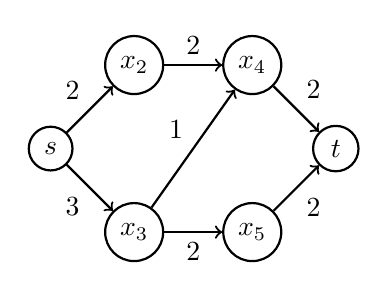
\begin{tikzpicture}[node distance={15mm}, thick, main/.style = {draw, circle}]
                \node[main] (1) {$s$};
                \node[main] (2) [above right of=1] {$x_2$};
                \node[main] (3) [below right of=1] {$x_3$};
                \node[main] (4) [right of=2] {$x_4$};
                \node[main] (5) [right of=3] {$x_5$};
                \node[main] (6) [above right of=5] {$t$};
                \draw[->] (1) -- node[midway, above left] {2} (2);
                \draw[->] (1) -- node[midway, below left] {3} (3);
                \draw[->] (2) -- node[midway, above] {2} (4);
                \draw[->] (3) -- node[midway, above left] {1} (4);
                \draw[->] (3) -- node[midway, below] {2} (5);
                \draw[->] (4) -- node[midway, above right] {2} (6);
                \draw[->] (5) -- node[midway, below right] {2} (6);
            \end{tikzpicture}\\
            Max flow: 4\\
            Add 1 to edge with minimum capacity\\
            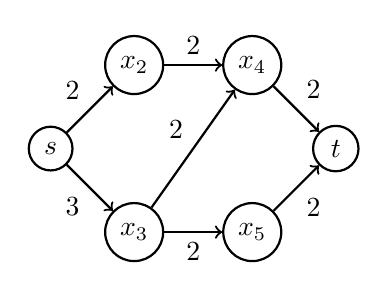
\begin{tikzpicture}[node distance={15mm}, thick, main/.style = {draw, circle}]
                \node[main] (1) {$s$};
                \node[main] (2) [above right of=1] {$x_2$};
                \node[main] (3) [below right of=1] {$x_3$};
                \node[main] (4) [right of=2] {$x_4$};
                \node[main] (5) [right of=3] {$x_5$};
                \node[main] (6) [above right of=5] {$t$};
                \draw[->] (1) -- node[midway, above left] {2} (2);
                \draw[->] (1) -- node[midway, below left] {3} (3);
                \draw[->] (2) -- node[midway, above] {2} (4);
                \draw[->] (3) -- node[midway, above left] {2} (4);
                \draw[->] (3) -- node[midway, below] {2} (5);
                \draw[->] (4) -- node[midway, above right] {2} (6);
                \draw[->] (5) -- node[midway, below right] {2} (6);
            \end{tikzpicture}\\
            However, the max flow remains the same since $x_4 \to t$ and $s \to x_3$ can't pass
            more flow\\
            % TODO
            \item \textbf{(2 point)}\\
            True, we can describe the max flow as the min-cut where $s \in A$ and $t \in B$\\
            Since the sum of integers divisible by 3 is divisible by 3, we can say that every cut
            is divisible by 3, and therefore the min-cut is also divisible by 3.\\
            Therefore, the max flow is divisible by 3.\\
            % TODO
            \item \textbf{(1 point)}\\
            False, it can still be unique\\
            Consider this graph:\\
            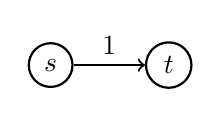
\begin{tikzpicture}[node distance={15mm}, thick, main/.style = {draw, circle}]
                \node[main] (1) {$s$};
                \node[main] (2) [right of=1] {$t$};
                \draw[->] (1) -- node[midway, above] {1} (2);
            \end{tikzpicture}\\
            There is one edge, so all edges have the same capacity\\
            There is only one possible min-cut, so it's unique\\
            % TODO
            \item \textbf{(2 points)}\\
            False, the min-cuts may change\\
            Consider the following graph:\\
            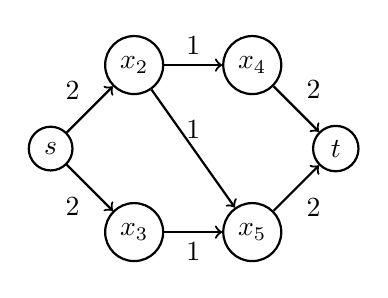
\begin{tikzpicture}[node distance={15mm}, thick, main/.style = {draw, circle}]
                \node[main] (1) {$s$};
                \node[main] (2) [above right of=1] {$x_2$};
                \node[main] (3) [below right of=1] {$x_3$};
                \node[main] (4) [right of=2] {$x_4$};
                \node[main] (5) [right of=3] {$x_5$};
                \node[main] (6) [above right of=5] {$t$};
                \draw[->] (1) -- node[midway, above left] {2} (2);
                \draw[->] (1) -- node[midway, below left] {2} (3);
                \draw[->] (2) -- node[midway, above] {1} (4);
                \draw[->] (2) -- node[midway, above] {1} (5);
                \draw[->] (3) -- node[midway, below] {1} (5);
                \draw[->] (4) -- node[midway, above right] {2} (6);
                \draw[->] (5) -- node[midway, below right] {2} (6);
            \end{tikzpicture}\\
            The min-cuts are $\{s, x_3\}$ and $\{x_2, x_4, x_5, t\}$ with a capacity of 3 and
            $\{s, x_2, x_3\}$ and $\{x_4, x_5, t\}$ with a capacity of 3 and $\{s, x_2, x_3, x_5\}$
            and $\{x_4, t\}$ with a capacity of 3\\
            Let's add 2 to all edges\\
            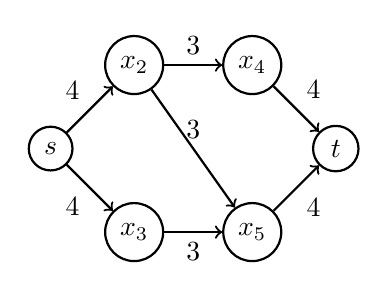
\begin{tikzpicture}[node distance={15mm}, thick, main/.style = {draw, circle}]
                \node[main] (1) {$s$};
                \node[main] (2) [above right of=1] {$x_2$};
                \node[main] (3) [below right of=1] {$x_3$};
                \node[main] (4) [right of=2] {$x_4$};
                \node[main] (5) [right of=3] {$x_5$};
                \node[main] (6) [above right of=5] {$t$};
                \draw[->] (1) -- node[midway, above left] {4} (2);
                \draw[->] (1) -- node[midway, below left] {4} (3);
                \draw[->] (2) -- node[midway, above] {3} (4);
                \draw[->] (2) -- node[midway, above] {3} (5);
                \draw[->] (3) -- node[midway, below] {3} (5);
                \draw[->] (4) -- node[midway, above right] {4} (6);
                \draw[->] (5) -- node[midway, below right] {4} (6);
            \end{tikzpicture}\\
            However, the min-cuts are now $\{s, x_3\}$ and $\{x_2, x_4, x_5, t\}$ with a
            capacity of 7 and $\{s, x_2, x_3, x_5\}$ and $\{x_4, t\}$ with a capacity of 7\\
            % TODO
            \item \textbf{(2 points)}\\
            True, the min-cuts stay the same\\
            Assume this is false\\
            Now we have 2 cases: A min-cut previously is no longer a min-cut, or a new min-cut is
            added to the sets\\
            Assume a previous min-cut is no longer a min-cut, lets call it $\alpha$\\
            Then, some other cut, lets call it $\beta$ has a smaller capacity than $\alpha$\\
            $\therefore$, $cap(\beta) < cap(\alpha)$, and since every edge was multiplied by a
            constant factor c, then this implies $\frac{cap(\beta)}{c} < \frac{cap(\alpha)}{c}$\\
            However, $\alpha$ was a min-cut before, so $\frac{cap(\beta)}{c} \geq \frac{cap(\alpha)
            }{c}$\\
            This is a contradiction, so a previous min-cut can't be no longer a min-cut\\
            Now for the second case, assume a new min-cut is added to the sets, lets call it $\gamma$\\
            Therefore, for every cut $\xi$ in the transformed graph, $cap(\gamma) \leq cap(\xi)$\\
            Divide both sides by c, which yields $\frac{cap(\gamma)}{c} \leq \frac{cap(\xi)}{c}$\\
            This means that $\gamma$ is a min-cut in the original graph, which is a contradiction\\
            Therefore, the min-cuts stay the same\\
            % TODO
            \item \textbf{(2 points)}\\
            False, the max flow may change\\
            Consider the following graph:\\
            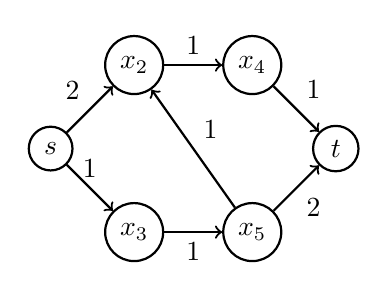
\begin{tikzpicture}[node distance={15mm}, thick, main/.style = {draw, circle}]
                \node[main] (1) {$s$};
                \node[main] (2) [above right of=1] {$x_2$};
                \node[main] (3) [below right of=1] {$x_3$};
                \node[main] (4) [right of=2] {$x_4$};
                \node[main] (5) [right of=3] {$x_5$};
                \node[main] (6) [above right of=5] {$t$};
                \draw[->] (1) -- node[midway, above left] {2} (2);
                \draw[->] (1) -- node[midway, above] {1} (3);
                \draw[->] (2) -- node[midway, above] {1} (4);
                \draw[->] (3) -- node[midway, below] {1} (5);
                \draw[->] (4) -- node[midway, above right] {1} (6);
                \draw[->] (5) -- node[midway, above right] {1} (2);
                \draw[->] (5) -- node[midway, below right] {2} (6);
            \end{tikzpicture}\\
            The max-flow is 2\\
            Now we transform this directed graph to an undirected graph\\
            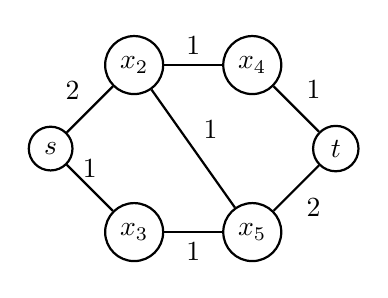
\begin{tikzpicture}[node distance={15mm}, thick, main/.style = {draw, circle}]
                \node[main] (1) {$s$};
                \node[main] (2) [above right of=1] {$x_2$};
                \node[main] (3) [below right of=1] {$x_3$};
                \node[main] (4) [right of=2] {$x_4$};
                \node[main] (5) [right of=3] {$x_5$};
                \node[main] (6) [above right of=5] {$t$};
                \draw (1) -- node[midway, above left] {2} (2);
                \draw (1) -- node[midway, above] {1} (3);
                \draw (2) -- node[midway, above] {1} (4);
                \draw (3) -- node[midway, below] {1} (5);
                \draw (4) -- node[midway, above right] {1} (6);
                \draw (5) -- node[midway, above right] {1} (2);
                \draw (5) -- node[midway, below right] {2} (6);
            \end{tikzpicture}\\
            The max flow is now 3\\
            % TODO
        \end{enumerate}
    \end{homeworkProblem}

    \begin{homeworkProblem}
        \textbf{(10 points)}
        % TODO
    \end{homeworkProblem}

    \begin{homeworkProblem}
        \textbf{(10 points)}
        % TODO
    \end{homeworkProblem}
\end{document}
